\scalebox{0.8}{
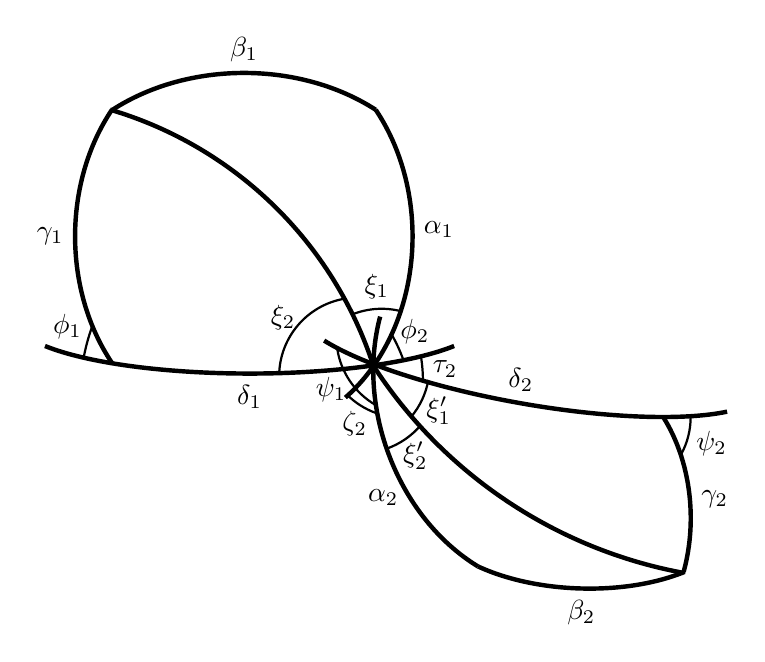
\begin{tikzpicture}
     \draw[ultra thick] (0.5, 2) arc[start angle=210, end angle = 330, x radius = 3cm, y radius = 0.7cm]  node[below, midway] {$\delta_1$};
        \draw[ultra thick] (1.35, 5) arc [start angle=140, end angle=220,x radius = 2cm, y radius = 2.5cm] node[left, midway] {$\gamma_1$};
        \draw[ultra thick] (4.7, 5) arc [start angle=40, end angle=-55,x radius = 2cm, y radius = 2.5cm] node[right, pos = 0.4] {$\alpha_1$};
        \draw[ultra thick] (4.7,5) arc [start angle=50, end angle=130,x radius =2.6cm, y radius = 2cm] node[above, midway] {$\beta_1$};
        \draw[thick] (1.1, 2.25) arc[start angle = 160, end angle = 170,radius=2.5cm] node[left, pos = 0] {$\phi_1$};
        \draw[thick] (4.9, 2.15) arc[start angle = 30, end angle = 20,radius=2cm] node[right, pos = -0.1] {$\phi_2$};
        
%        \node [red] at (11.7, 1.75) {\textbullet};
%        \node [red] at (15.35, 1.1) {\textbullet};
%        \node [green] at (13,-0.8) {\textbullet};
 %       \node [green] at (11.8, 1) {\textbullet};
        
        
        \draw[ultra thick, rotate around={-10:(4.7,1.75)}] (4, 1.95) arc [start angle=210, end angle = 330, x radius = 3cm, y radius = 0.7cm] node[above, midway] {$\delta_2$};
        \draw[ultra thick, rotate around = {19:(6,-0.8)}] (6,-0.8) arc [start angle=-134, end angle=-220,x radius = 2cm, y radius = 2.5cm] node[left, pos = 0.35] {$\alpha_2$};
        \draw[ultra thick, rotate around = {0:(8.35,1.1)}] (8.35,1.1) arc [start angle=40, end angle=-20,x radius = 1.5cm, y radius = 2cm] node[right, pos = 0.55] {$\gamma_2$};
        \draw[ultra thick, rotate around = {-2:(6,-0.8)}] (6,-0.8) arc [start angle=230, end angle=312,x radius = 2cm, y radius = 1cm] node[below, midway] {$\beta_2$};
        \draw[thick] (5.3, 1.55) arc[start angle = 0, end angle = 9,radius=2cm] node[right, pos = 0.5] {$\tau_2$};
        \draw[thick] (4.7, 1.25) arc[start angle = -120, end angle = -171,radius=1cm] node[left, pos = 0.35] {$\psi_1$};
        \draw[thick] (8.7, 1.1) arc[start angle = 0, end angle = -28, radius=1cm] node[right, pos = 0.7] {$\psi_2$};
        \draw[thick] (4.7, 1.15) arc[start angle = -110, end angle = -135, radius=1cm] node[below, pos = 0.7] {$\zeta_2$};
        \draw[ultra thick, rotate around = {18:(4.67, 1.75)}] (4.67, 1.75) arc[start angle = 0, end angle = 55.6, radius = 5cm];
        \draw[ultra thick, rotate around = {-147:(4.67, 1.75)}] (4.67, 1.75) arc[start angle = 0, end angle = 46.5, radius = 6cm];
        \draw[thick] (4.4, 2.4) arc[start angle = 112, end angle = 75, radius = 1cm] node[above, pos = 0.5] {$\xi_1$};
        \draw[thick] (4.3, 2.6) arc[start angle = 100, end angle = 179, radius = 1cm] node[left, pos = 0.4] {$\xi_2$};
        \draw[thick] (5.15, 1.1) arc[start angle = -40, end angle = -10, radius = 1cm]  node[right, pos = 0.2] {$\xi'_1$};
        \draw[thick] (4.85, 0.7) arc[start angle = -70, end angle = -40, radius = 1cm]  node[below, pos = 0.8] {$\xi'_2$};
    \end{tikzpicture}
}